\documentclass[11pt]{article}
\usepackage{geometry} % Pour passer au format A4
\geometry{hmargin=1cm, vmargin=1cm} % 

% Page et encodage
\usepackage[T1]{fontenc} % Use 8-bit encoding that has 256 glyphs
\usepackage[english,french]{babel} % Français et anglais
\usepackage[utf8]{inputenc} 

\usepackage{lmodern}
\setlength\parindent{0pt}

% Graphiques
\usepackage{graphicx,float,grffile}

% Maths et divers
\usepackage{amsmath,amsfonts,amssymb,amsthm,verbatim}
\usepackage{multicol,enumitem,url,eurosym,gensymb}

% Sections
\usepackage{sectsty} % Allows customizing section commands
\allsectionsfont{\centering \normalfont\scshape}

% Tête et pied de page

\usepackage{fancyhdr} 
\pagestyle{fancyplain} 

\fancyhead{} % No page header
\fancyfoot{}

\renewcommand{\headrulewidth}{0pt} % Remove header underlines
\renewcommand{\footrulewidth}{0pt} % Remove footer underlines

\newcommand{\horrule}[1]{\rule{\linewidth}{#1}} % Create horizontal rule command with 1 argument of height

\newcommand{\tempsexo}[1]{\textit{\textbf{(#1)}}}
%----------------------------------------------------------------------------------------
%   Début du document
%----------------------------------------------------------------------------------------

\begin{document}

%----------------------------------------------------------------------------------------
% RE-DEFINITION
%----------------------------------------------------------------------------------------
% MATHS
%-----------

\newtheorem{Definition}{Définition}
\newtheorem{Theorem}{Théorème}
\newtheorem{Proposition}{Propriété}
\newtheorem{Exo}{Éxercice}

% MATHS
%-----------
\renewcommand{\labelitemi}{$\bullet$}
\renewcommand{\labelitemii}{$\circ$}
%----------------------------------------------------------------------------------------
%   Titre
%----------------------------------------------------------------------------------------

\setlength{\columnseprule}{1pt}

\section*{S2 : Correction - Semaine du 23/03 au 29/03}

\subsection*{Travail sur le chapitre - Fonctions linéaires}

\Exo{p124 ex14}\\
On considère la fonction f telle que $f(x) = -4x - 7$

\begin{multicols}{3}
\begin{enumerate}
    \item[a.] 8
    \begin{align*}
        f(x) &= -4x - 7 \\
        f(8) &= -4 \times 8 - 7 \\
        f(8) &= -39  
    \end{align*}\columnbreak

    \item[b.]  -4
    \begin{align*}
        f(x) &= -4x - 7 \\
        f(-4) &= -4 \times (-4) - 7 \\
        f(-4) &= 9
    \end{align*}\columnbreak

    \item[c.]  -2
    \begin{align*}
        f(x) &= -4x - 7 \\
        f(-2) &= -4 \times (-2) - 7 \\
        f(-2) &= 1
    \end{align*}

\end{enumerate}
 \end{multicols}

\begin{multicols}{2}
\begin{enumerate}
     \item[d.]   $\dfrac{3}{2}$
    \begin{align*}
        f(x) &= -4x - 7 \\
        f(\dfrac{3}{2}) &= -4 \times \dfrac{3}{2} - 7 \\
        f(\dfrac{3}{2}) &= -13
    \end{align*}\columnbreak

     \item[e.]   $- \dfrac{1}{3}$
    \begin{align*}
        f(x) &= -4x - 7 \\
        f(- \dfrac{1}{3}) &= -4 \times (- \dfrac{1}{3}) - 7 \\
        f(- \dfrac{1}{3}) &= - \dfrac{17}{3}
    \end{align*}            
\end{enumerate}
\end{multicols}
Remarque : C'est également une bonne occasion pour utiliser la touche / fonction CALC de sa calculatrice.


\Exo{p124 ex15} \\
Les fonctions suivantes sont-elles des fonctions affines ?
\begin{enumerate}
    \item[a.] $f(x) = 6x - 3$ : \textbf{OUI}, on a bien un coefficient ($6$) qui multiplie x et on passe à l'origine par -3. 
    \item[b.] $g(x) = -4x^2$ : \textbf{NON}, on a bien un coefficient ($-4$) mais devant un $x^2$ et pas seulement $x$. \textit{(On vera au lycée que cette fonction est du second degré)}
    \item[c.] $h(x) = \dfrac{1}{x} + 7$ : \textbf{NON}, On passe bien par 7 à l'origine mais on a $\dfrac{1}{x}$ et pas $x$. \textit{(On vera au lycée que cette fonction est l'inverse)}
    \item[d.] $k(x) = \dfrac{x}{2} - 5$ : \textbf{OUI,} on a bien un coefficient ($\dfrac{1}{2}$) qui multiplie $x$ et on passe à l'origine par -5. 
\end{enumerate}

\Exo{p124 ex16} \\
Remarque : C'est également une bonne occasion pour utiliser géogébra en ligne : \url{https://www.geogebra.org/graphing}\\

\begin{minipage}[t]{0.7\textwidth}
  \begin{figure}[H]
        \centering
        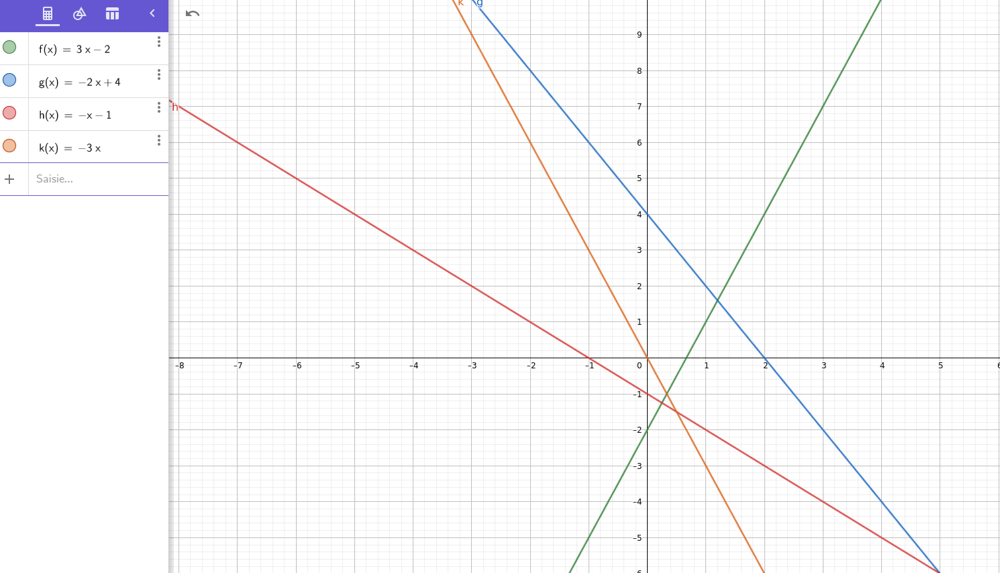
\includegraphics[width=0.9\linewidth]{_continuite/sources/s2-p124ex16.png}
  \end{figure}
\end{minipage}
\begin{minipage}[t]{0.3\textwidth}
\begin{enumerate}
    \item[a.] $f(x) = 3x - 2$
    \item[b.] $g(x) = -2x + 4$
    \item[c.] $h(x) = -x - 1$
    \item[d.] $k(x) = -3x$
\end{enumerate}
\end{minipage}

\newpage

\Exo{p124 ex16} \\

\begin{minipage}[t]{0.5\textwidth}
  \begin{figure}[H]
        \centering
        \includegraphics[width=0.9\linewidth]{_continuite/sources/s2-p124ex20.png}
  \end{figure}
\end{minipage}
\begin{minipage}[t]{0.5\textwidth}

\begin{enumerate}
    \item[a.] $d_1 : f(x) = -2x + 1$ \\
    La droite descend de 2 quand on avance de 1. : $a=-2$ et passe à l'origine par $1$. 
    \item[b.] $d_2 : g(x) = \dfrac{1}{2}x + 0 = \dfrac{x}{2}$\\
    La droite monte de 1 quand on avance de 2. : $a=\tfrac{1}{2}$ et passe à l'origine par $0$. 
    \item[c.] $d_3 : h(x) = 1x + 3 = x + 3$\\
    La droite monte de 1 quand on avance de 1. : $a=1$ et passe à l'origine par $3$. 
    \item[d.] $d_4 : k(x) = \dfrac{-5}{2}x + 5$\\
    La droite descend de 5 quand on avance de 2. : $a=\tfrac{-5}{2}$ et passe à l'origine par $5$. 
\end{enumerate}
\end{minipage}


\end{document}